\clearpage
\appendix
\section{Appendix}
\label{app:A}

 The measured values of the 
 branching fraction of the \decay{\Lb}{\Lz\mumu} decay normalised to
 \decay{\Lb}{\jpsi\Lz} decays are given in Table~\ref{tab:RelBR},
 where the statistical and total systematic uncertainties are shown
 separately. 

\begin{table}[th]
\centering
\renewcommand{\arraystretch}{1.2}
\caption{Differential branching fraction of the \decay{\Lb}{\Lz\mumu}
  decay relative to \decay{\Lb}{\jpsi\Lz} decays,
 where the uncertainties are statistical and systematic, respectively.}
\begin{tabular}{cccccc}
  \qsq interval  [\gevgevcccc] & &\multicolumn{4}{c}{ $\frac{\deriv\BF(\decay{\Lb}{\Lz\mumu})/\deriv\qsq}{\BF(\decay{\Lb}{\jpsi\Lz})} \cdot 10^{-3} [(\gevgevcccc)^{-1}]$} \\
\hline
0.1 -- 2.0   & &0.56 & $^{+0.20}_{-0.17}$ & $^{+0.03}_{-0.03}$ & \\
2.0 -- 4.0   & &0.18 & $^{+0.18}_{-0.15}$ & $^{+0.01}_{-0.01}$ & \\
4.0 -- 6.0   & &0.04 & $^{+0.14}_{-0.04}$ & $^{+0.01}_{-0.01}$ & \\
6.0 -- 8.0   & &0.40 & $^{+0.20}_{-0.17}$ & $^{+0.01}_{-0.02}$ &\\
                                                 
11.0 -- 12.5 & &1.19 & $^{+0.24}_{-0.23}$ & $^{+0.04}_{-0.07}$& \\
15.0 -- 16.0 & &1.78 & $^{+0.31}_{-0.28}$ & $^{+0.08}_{-0.08}$&\\
16.0 -- 18.0 & &1.94 & $^{+0.23}_{-0.22}$ & $^{+0.04}_{-0.09}$&\\
18.0 -- 20.0 & &1.97 & $^{+0.23}_{-0.22}$ & $^{+0.10}_{-0.07}$&\\
              
\hline        
1.1--6.0   & &0.14 & $ ^{+0.10}_{-0.09}$& $^{+0.01}_{-0.01}$&\\
15.0--20.0 & &1.90 & $ ^{+0.14}_{-0.14}$& $^{+0.04}_{-0.06}$&\\
\end{tabular}
\label{tab:RelBR}
\end{table}

\newpage

\begin{figure}[htbp]
\centering
%%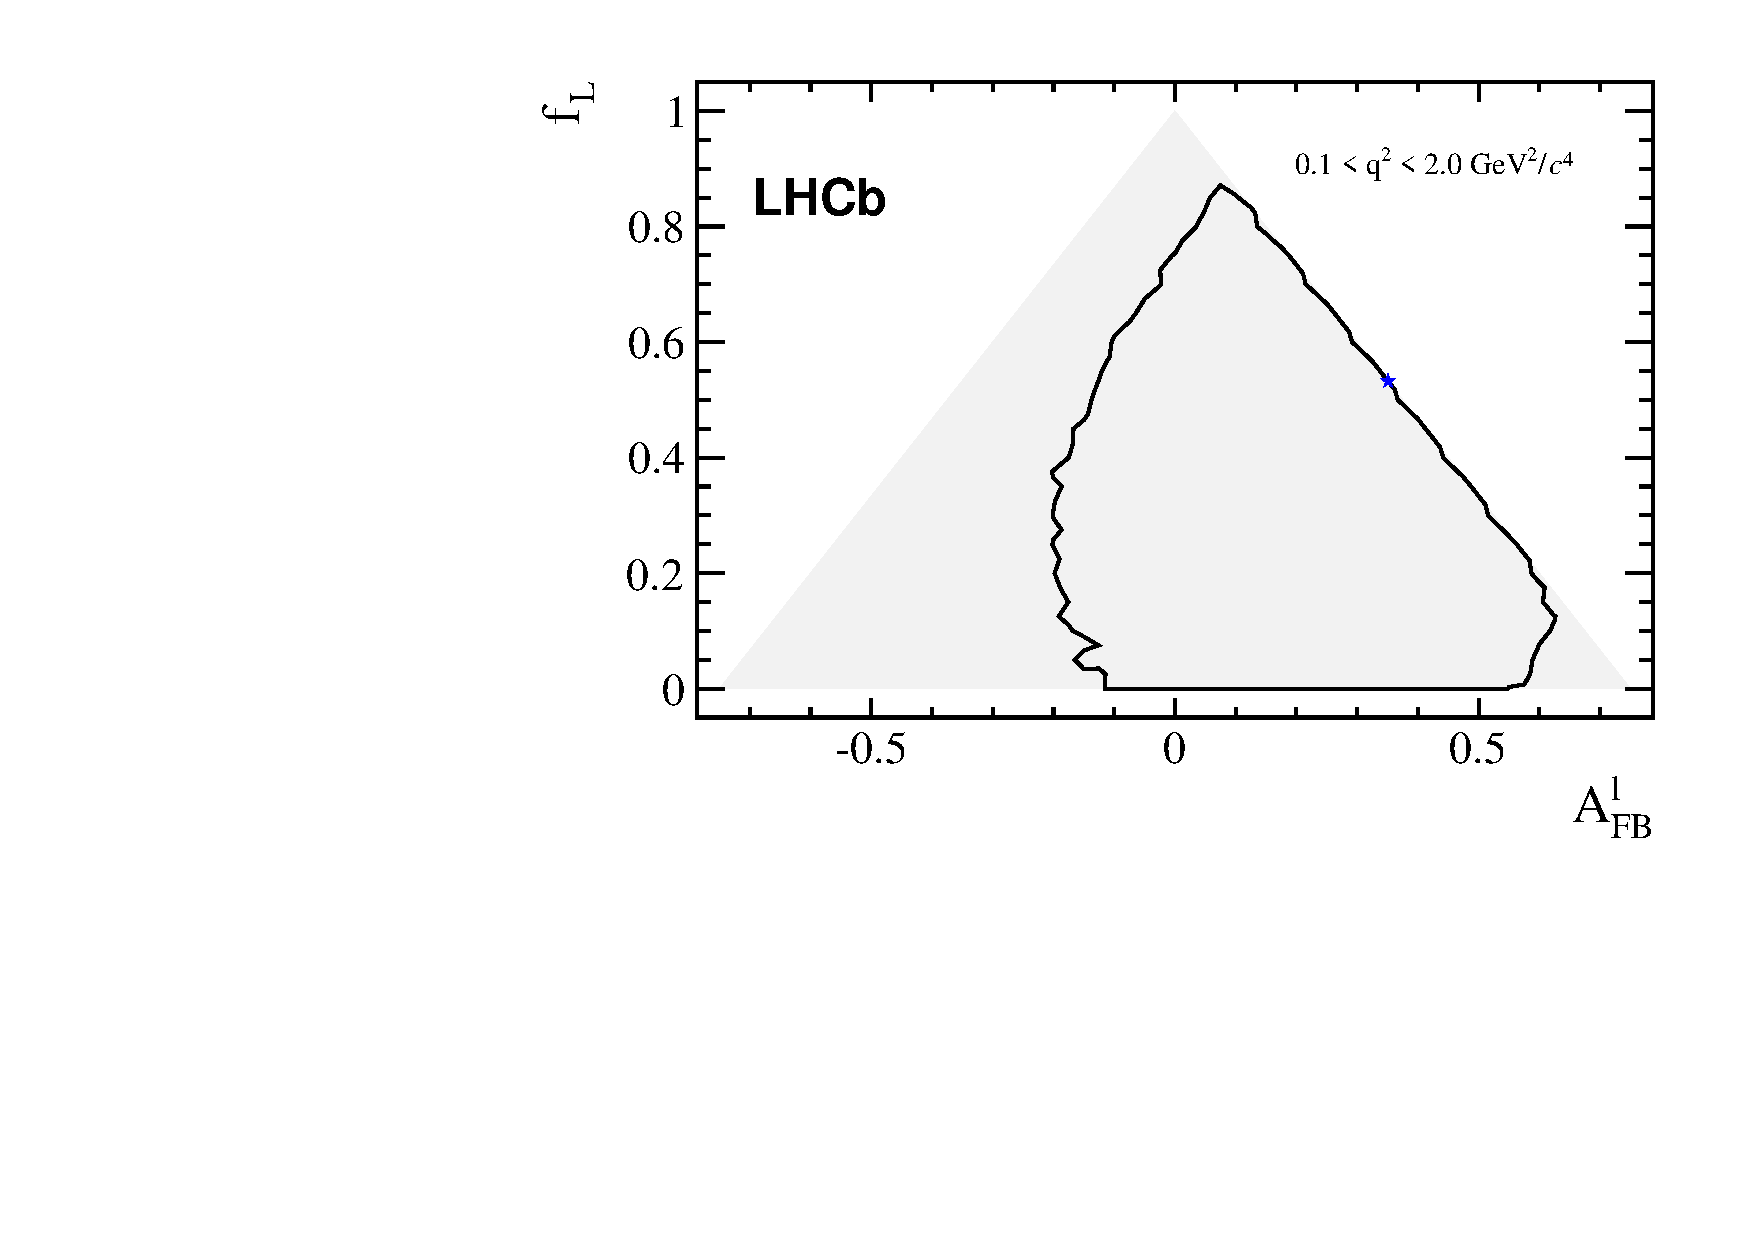
\includegraphics[width=0.49\textwidth]{images_and_tables/Angular/contours_010_200_1D.pdf}
%%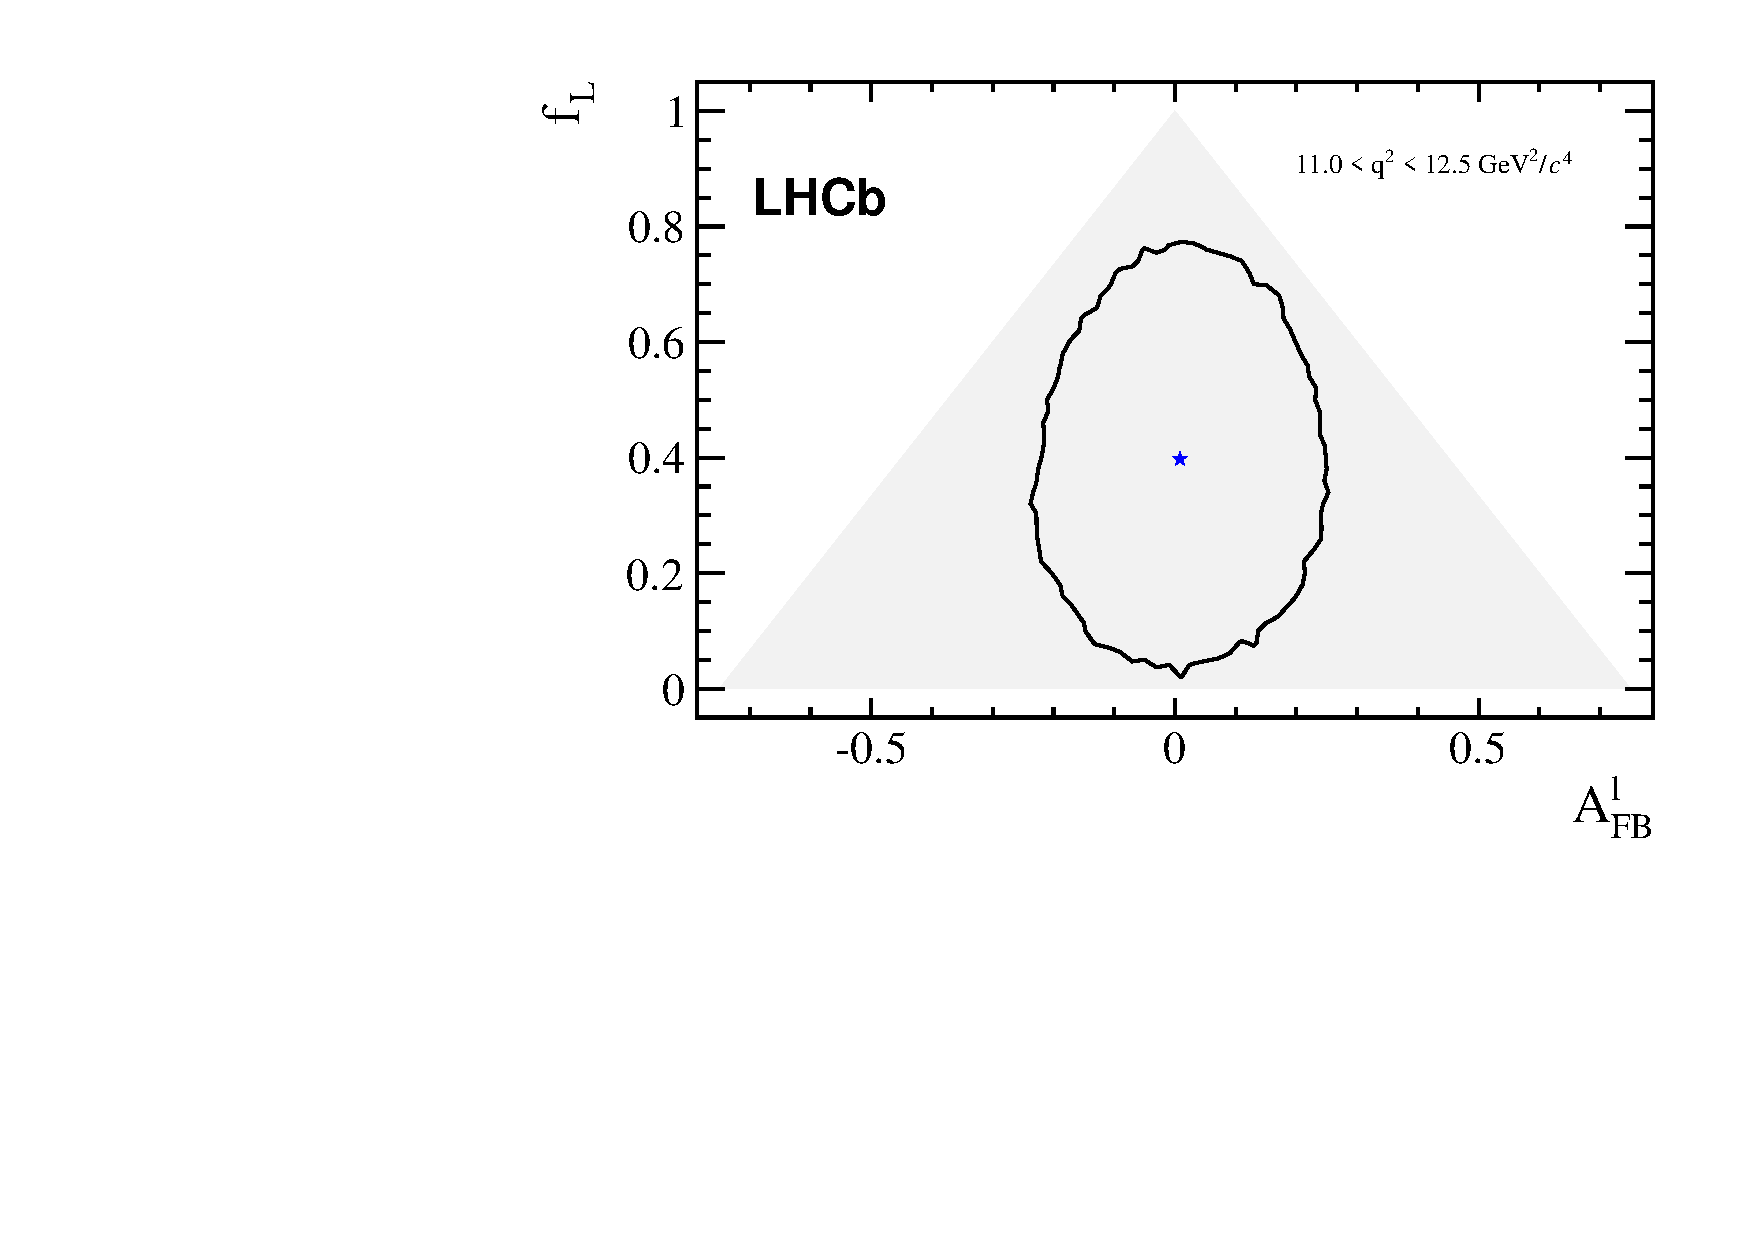
\includegraphics[width=0.49\textwidth]{images_and_tables/Angular/contours_1100_1250_1D.pdf}
%%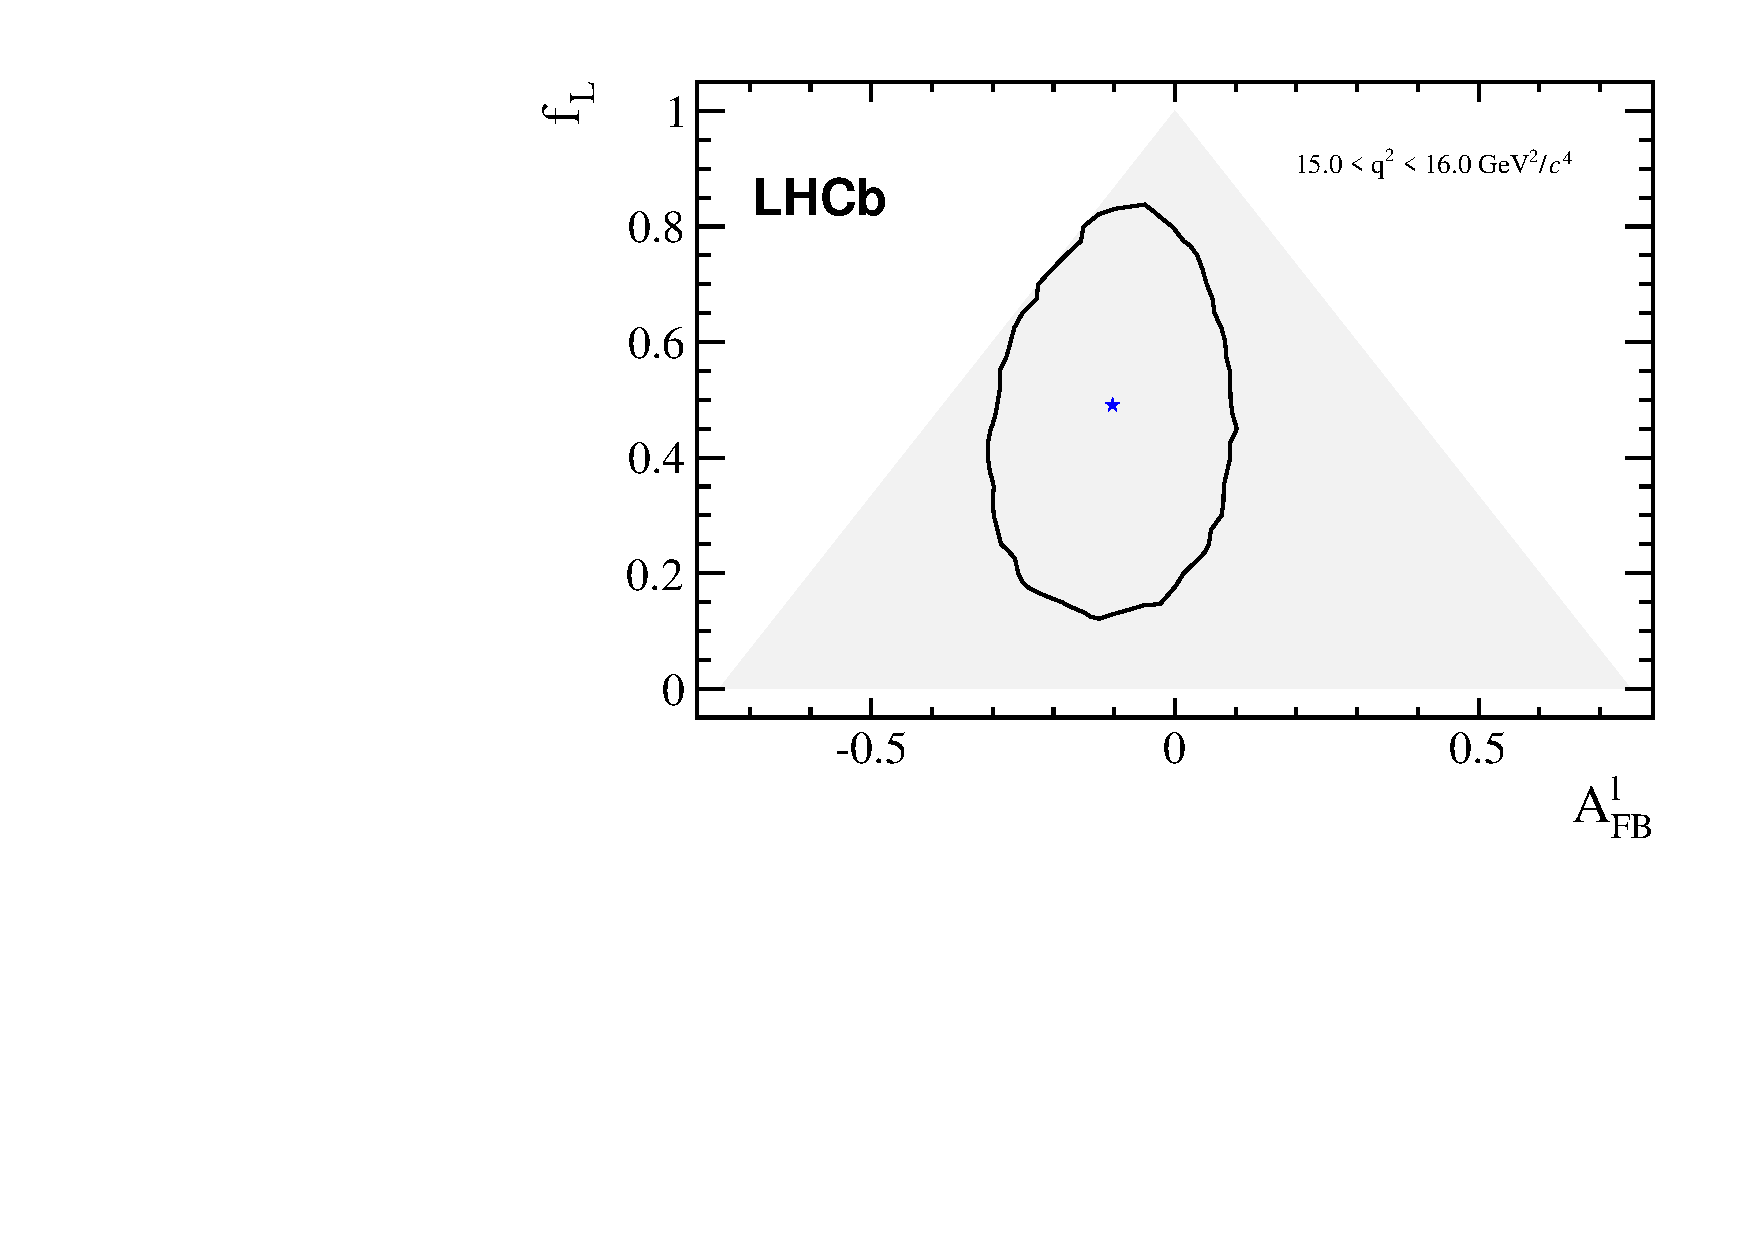
\includegraphics[width=0.49\textwidth]{images_and_tables/Angular/contours_1500_1600_1D.pdf}
%%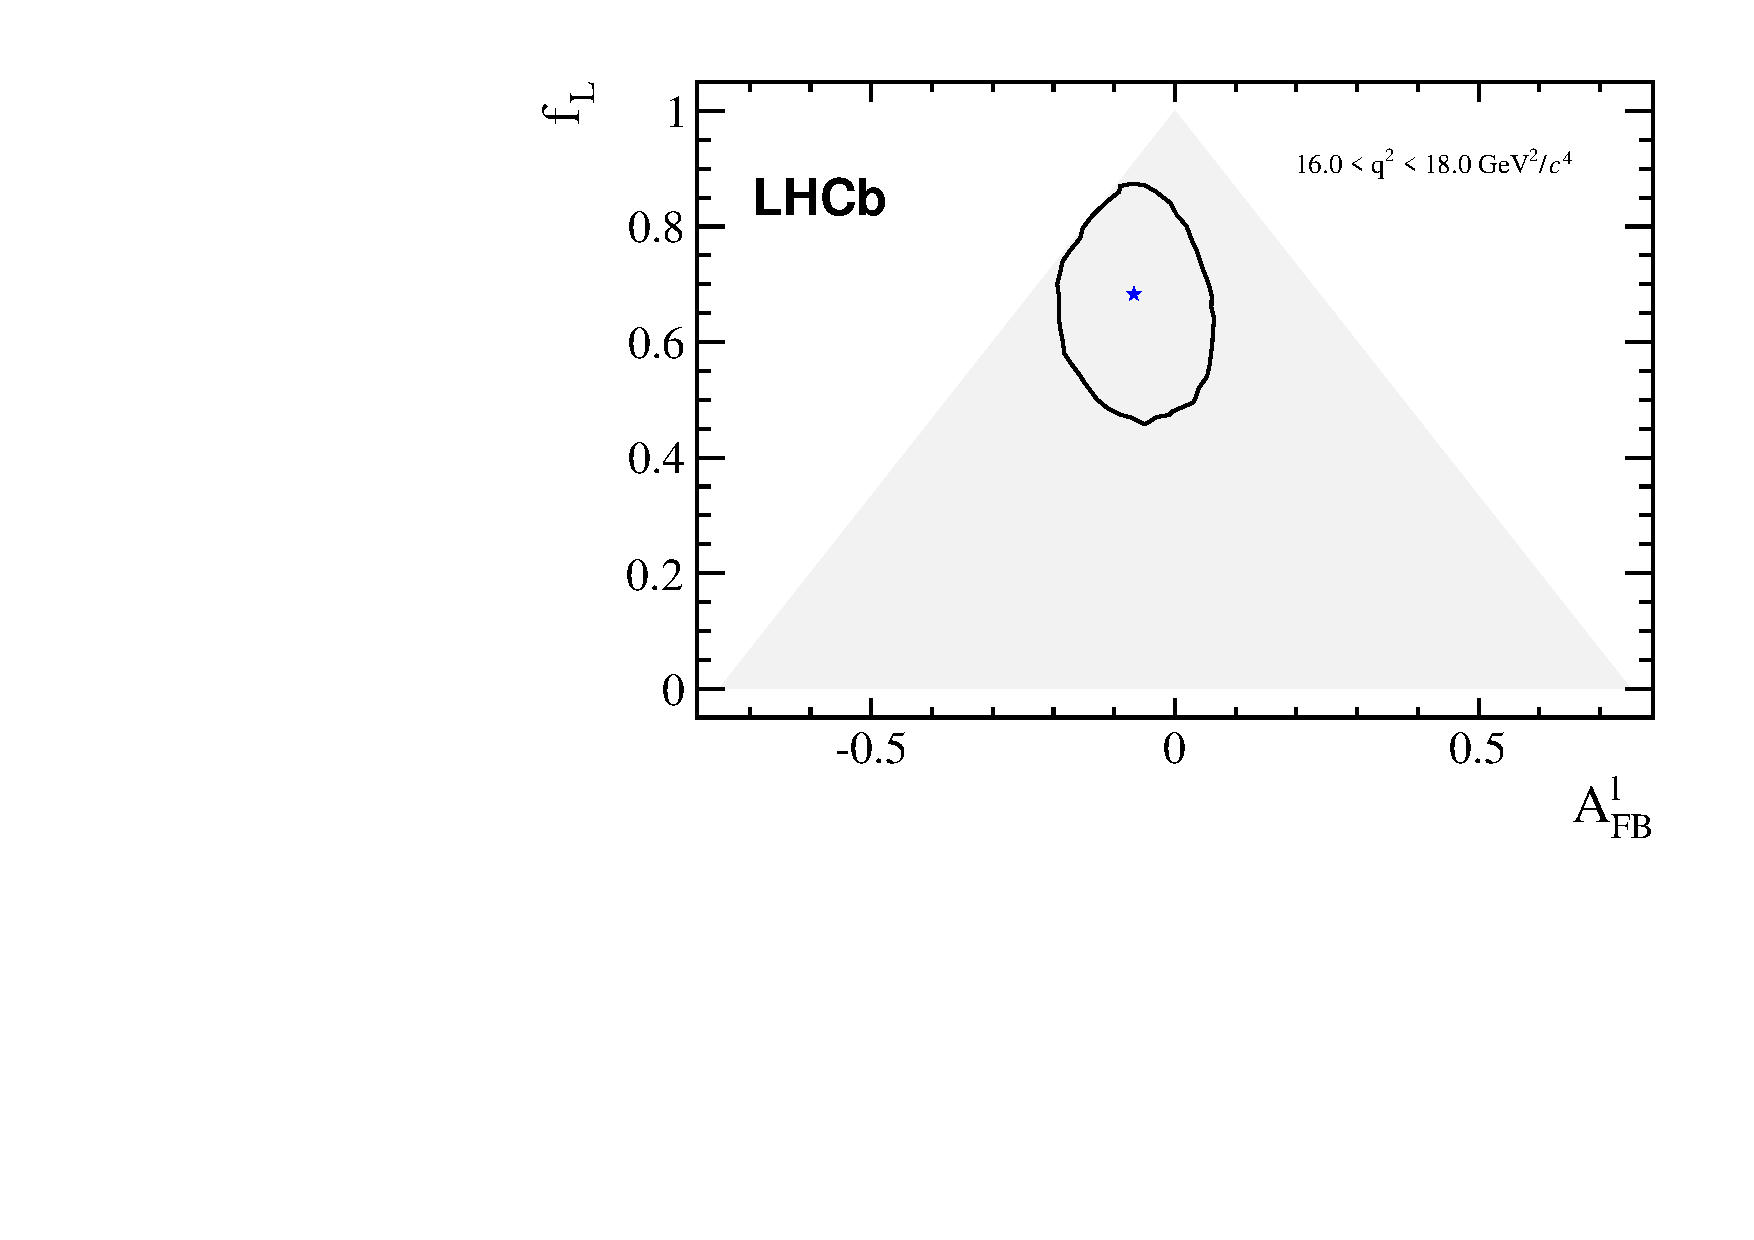
\includegraphics[width=0.49\textwidth]{images_and_tables/Angular/contours_1600_1800_1D.pdf}
%%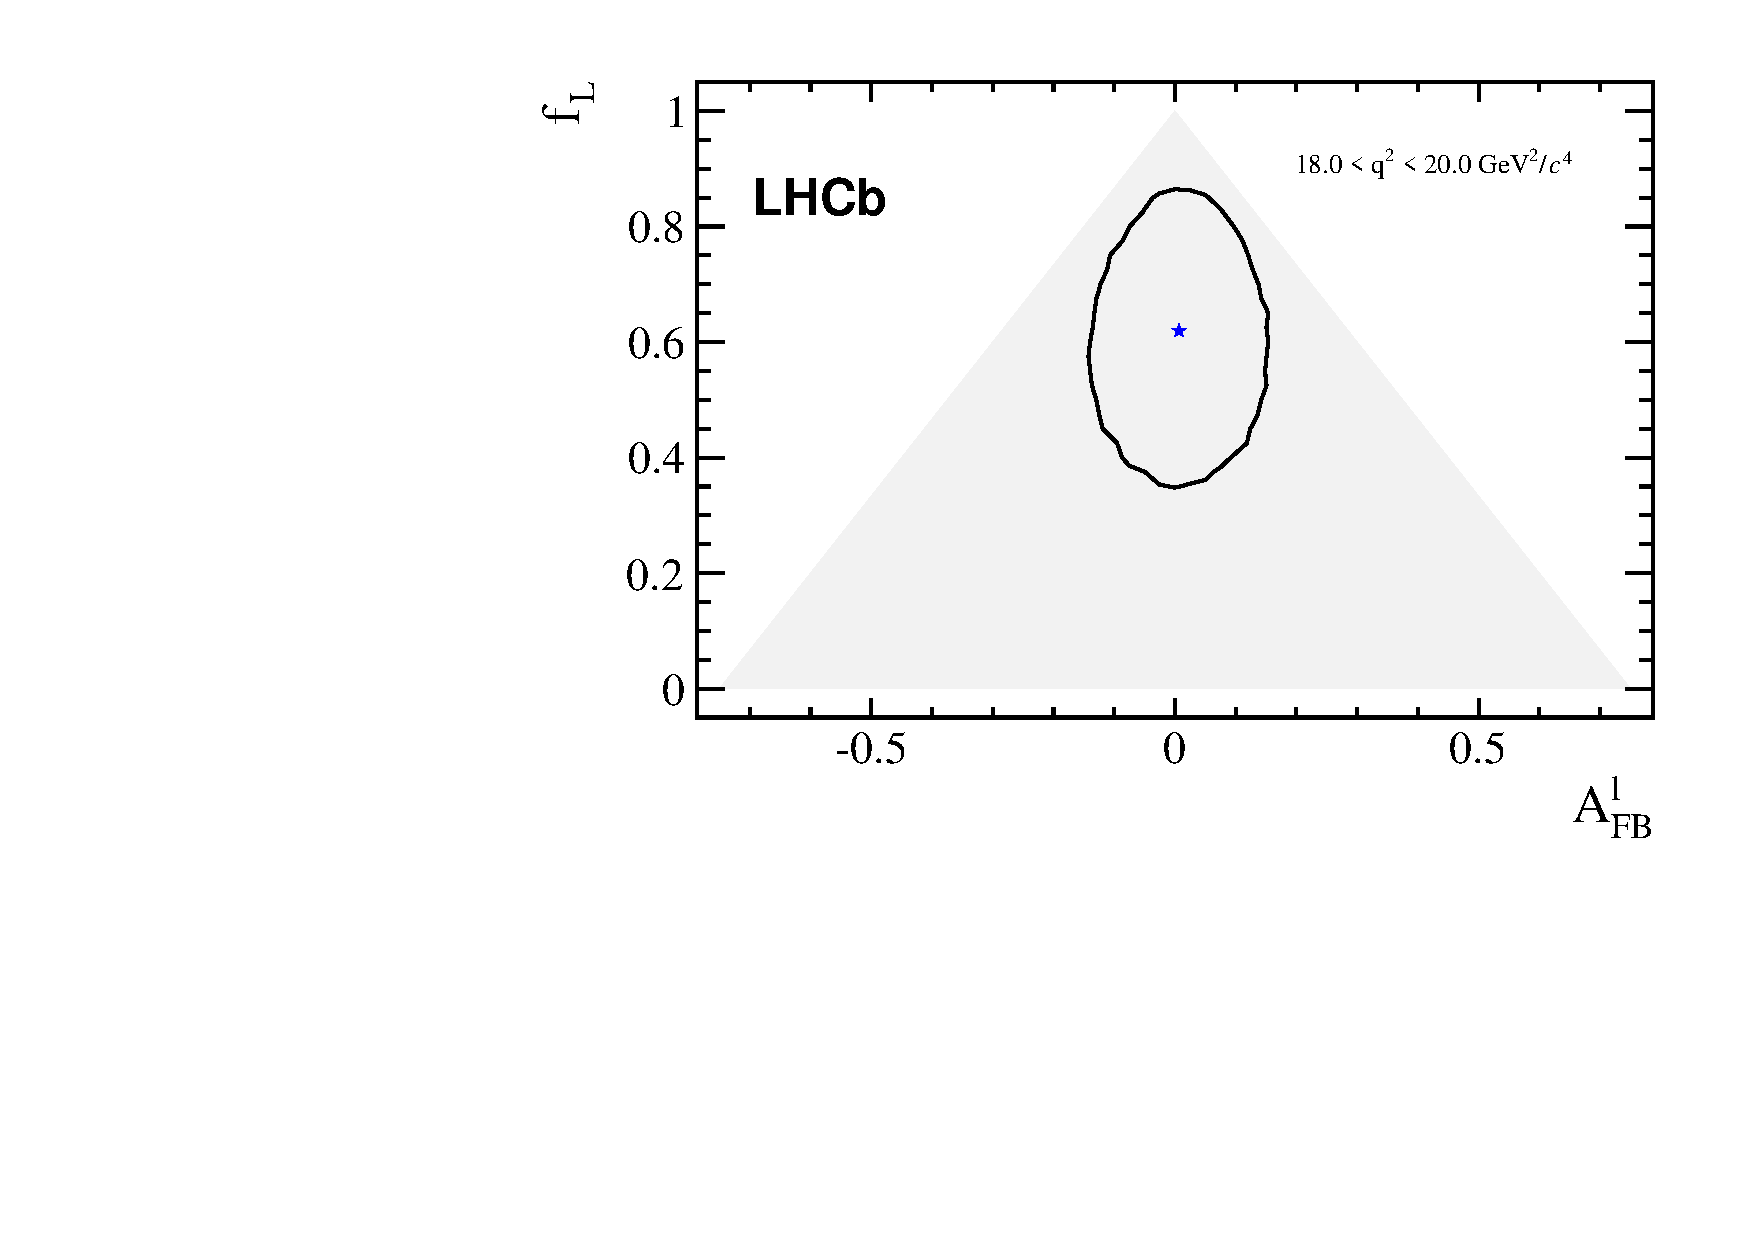
\includegraphics[width=0.49\textwidth]{images_and_tables/Angular/contours_1800_2000_1D.pdf}
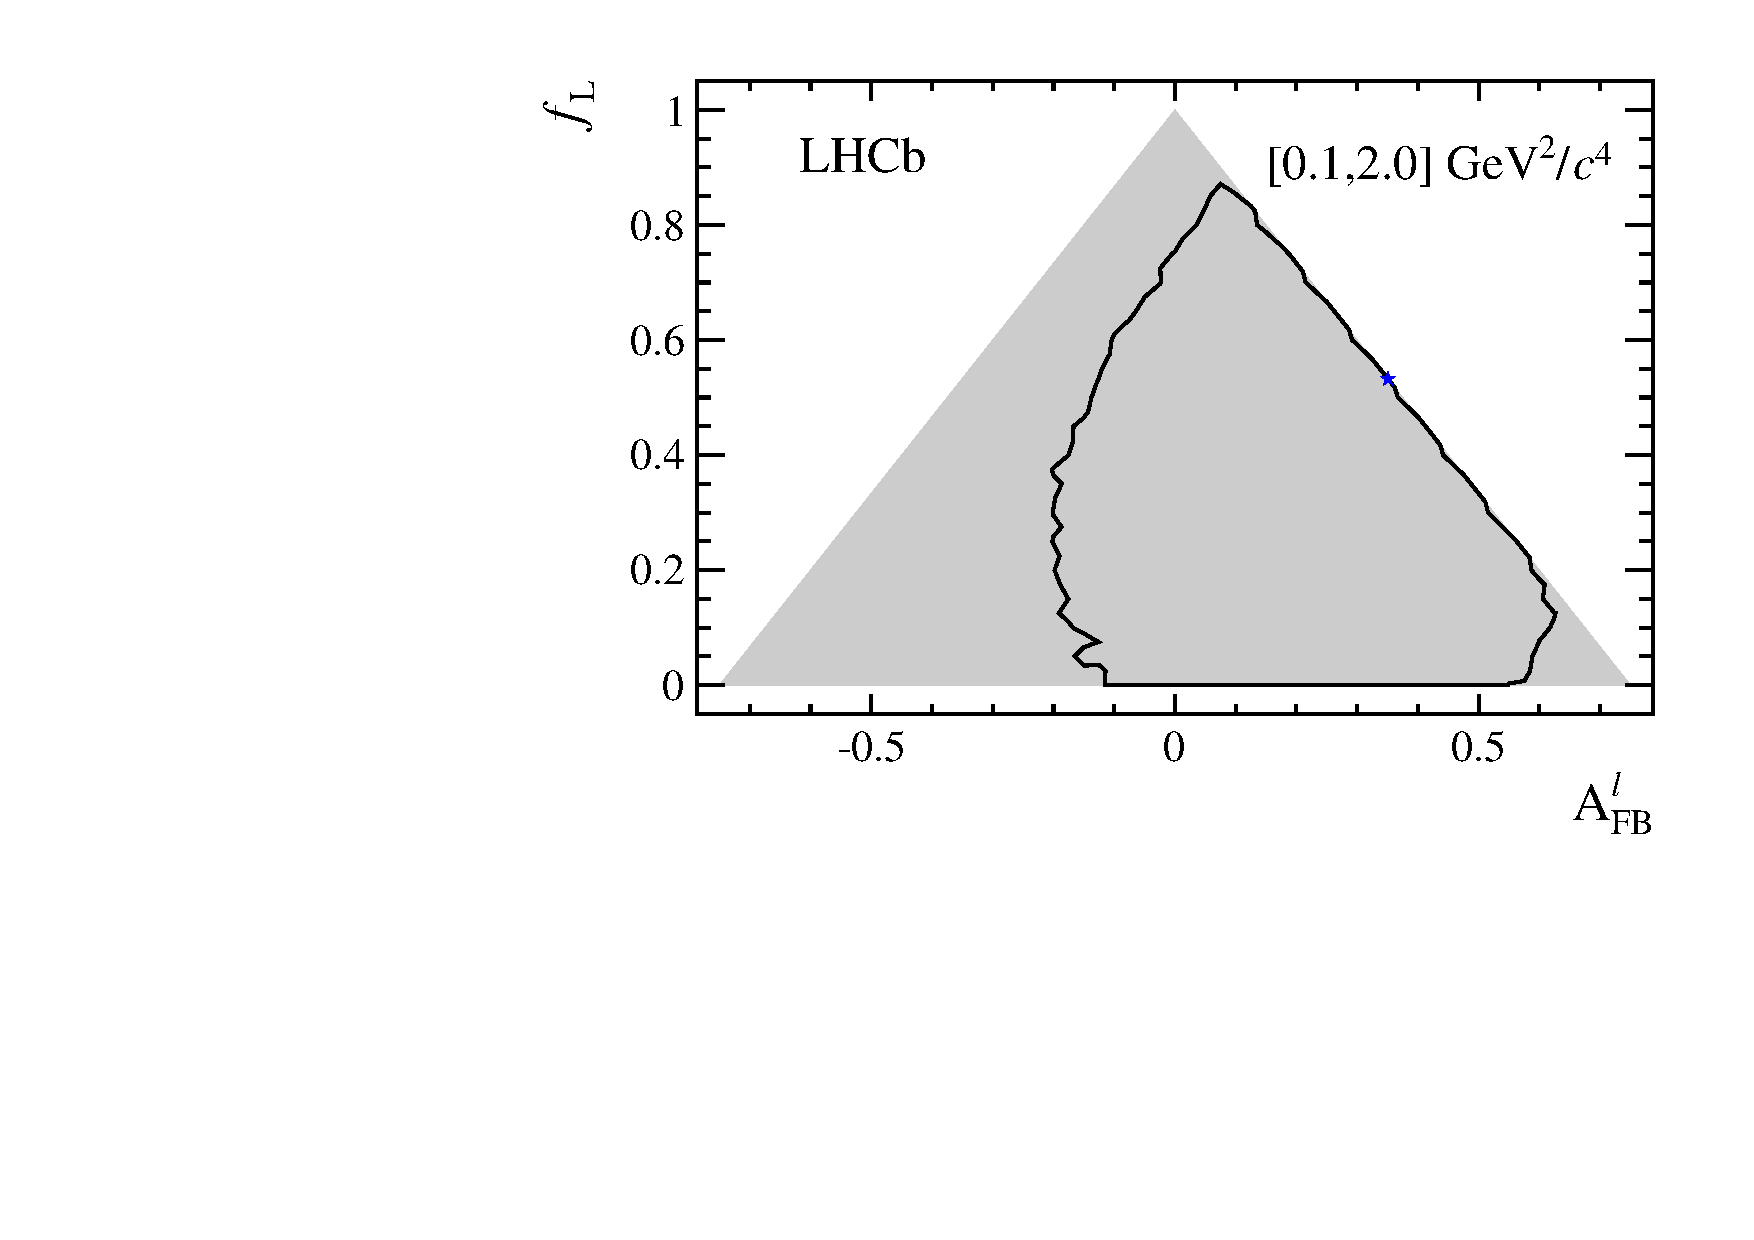
\includegraphics[width=0.49\textwidth]{figure10a.pdf}
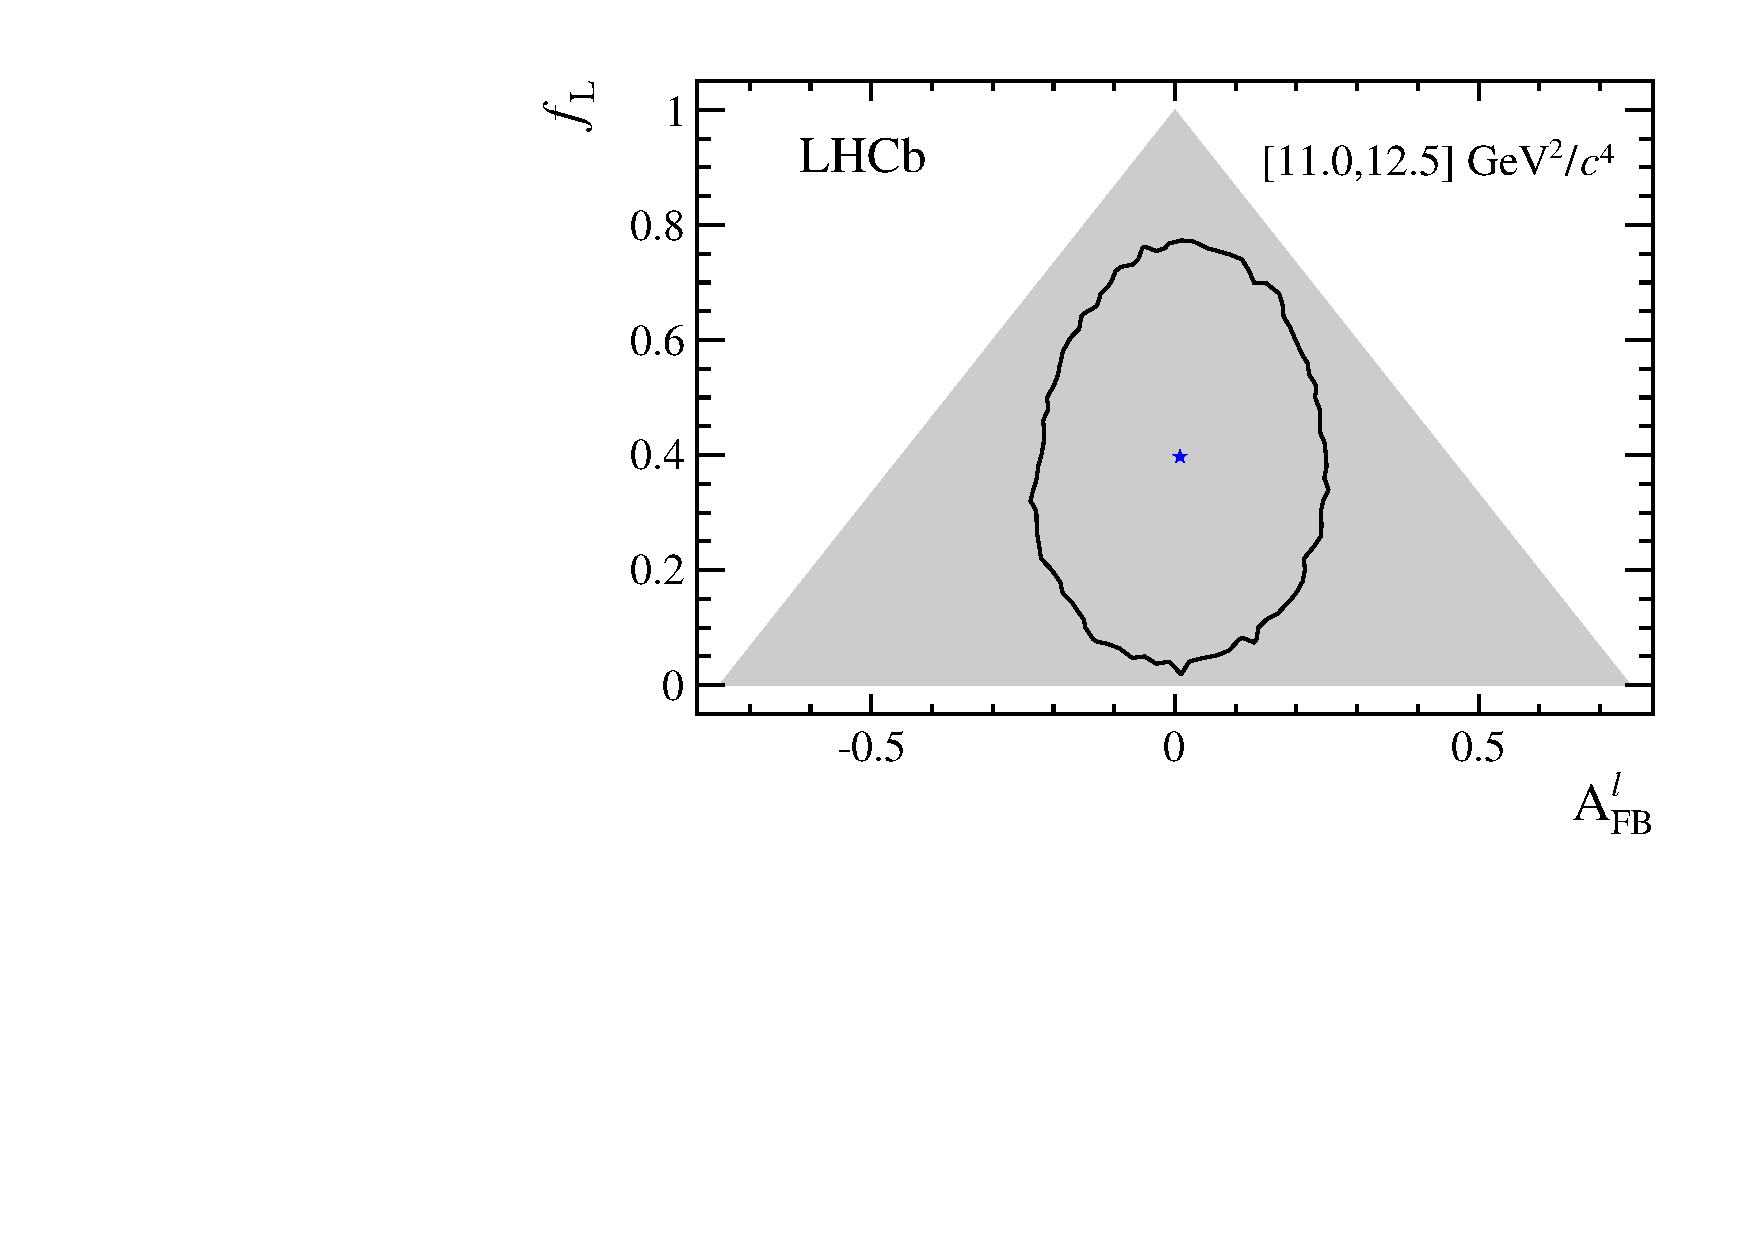
\includegraphics[width=0.49\textwidth]{figure10b.pdf}
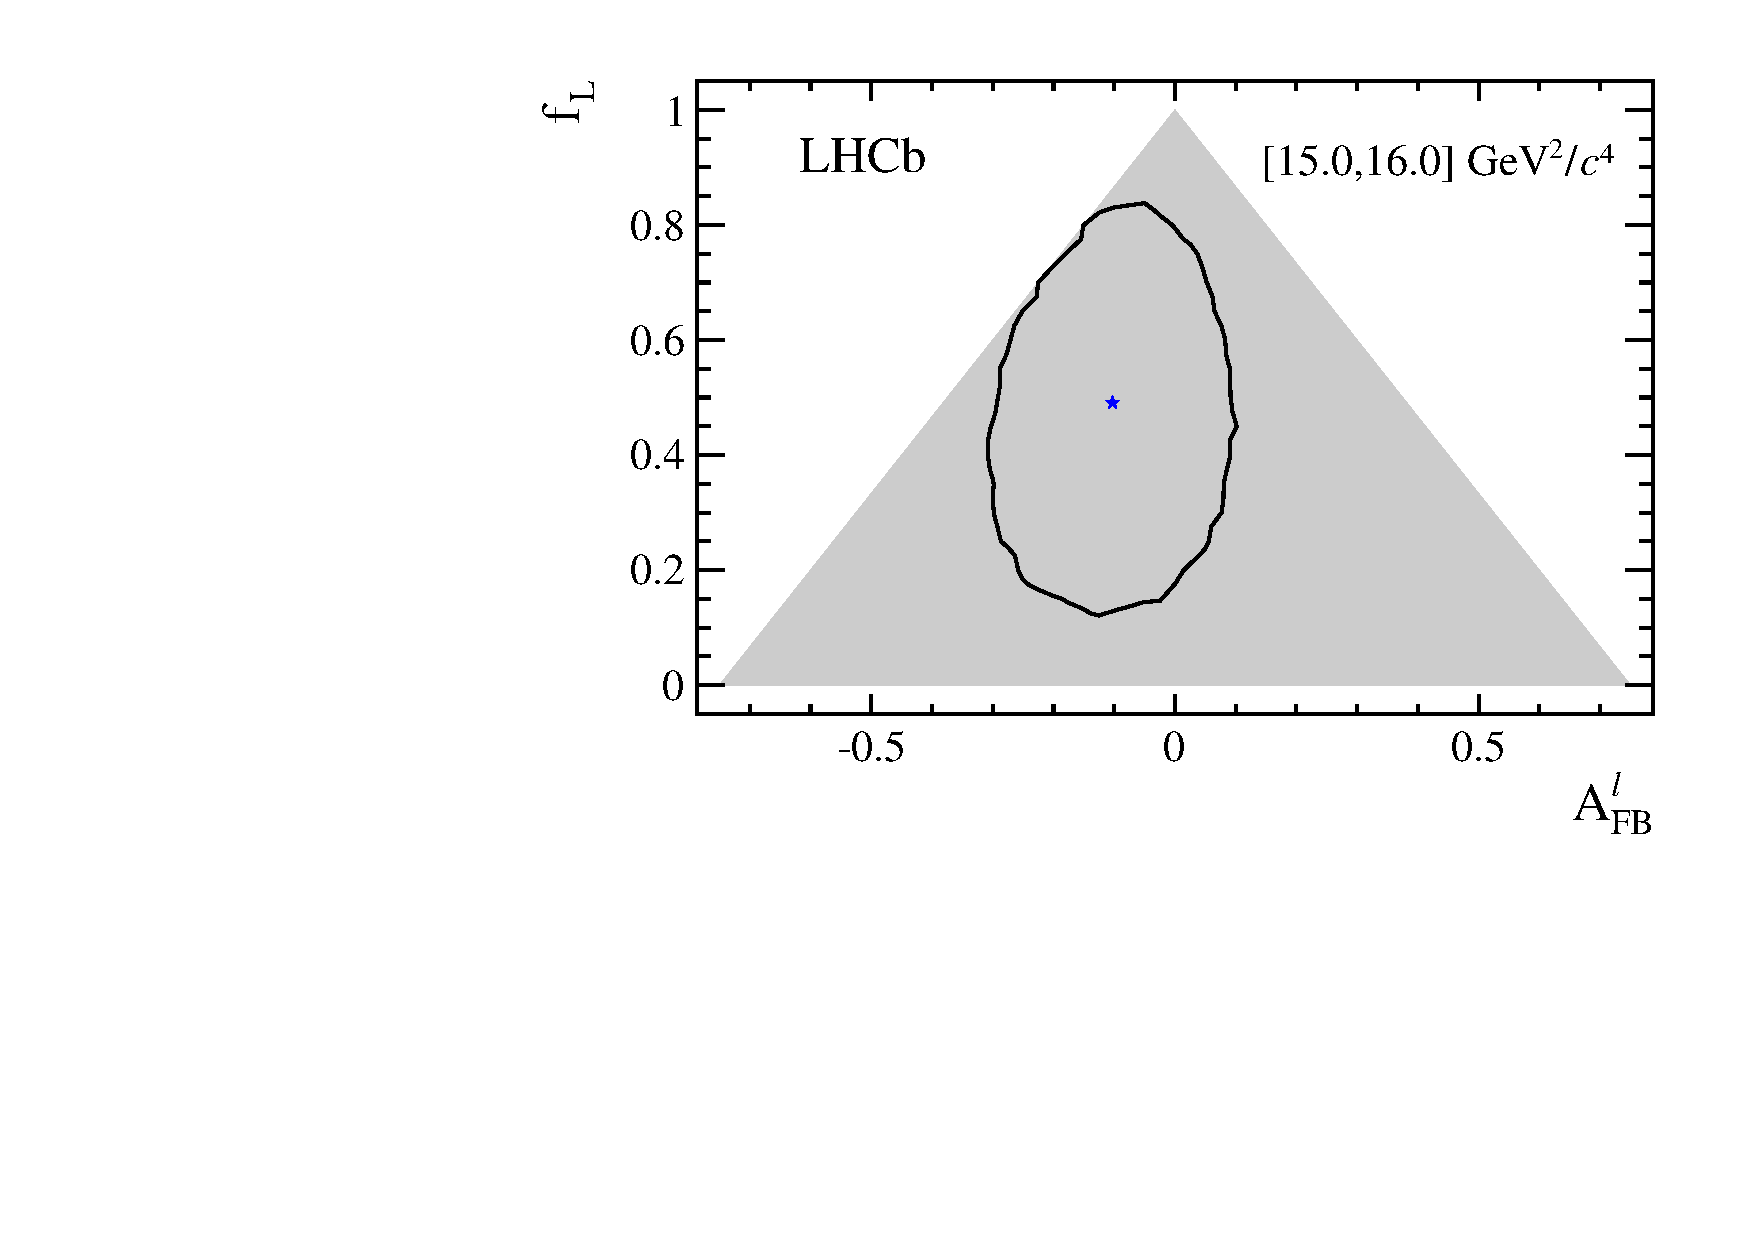
\includegraphics[width=0.49\textwidth]{figure10c.pdf}
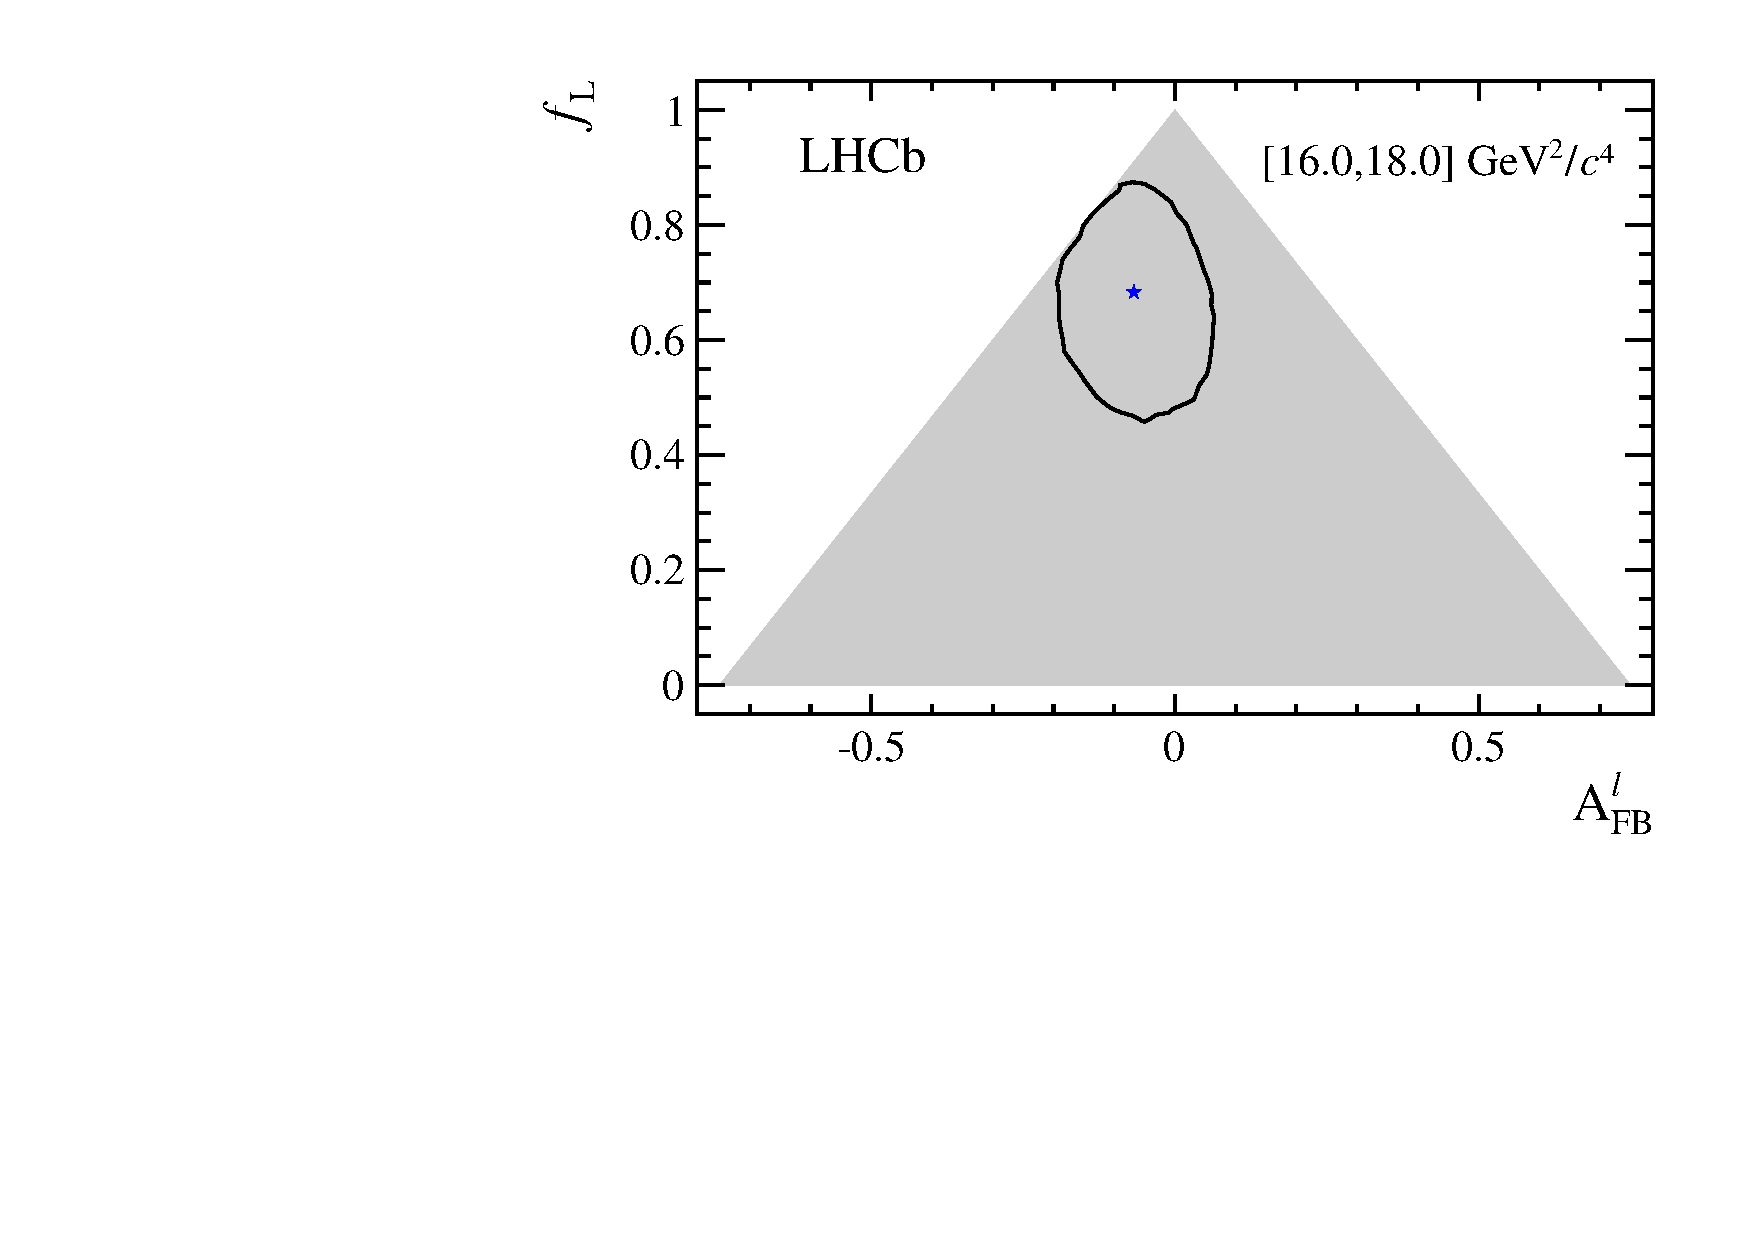
\includegraphics[width=0.49\textwidth]{figure10d.pdf}
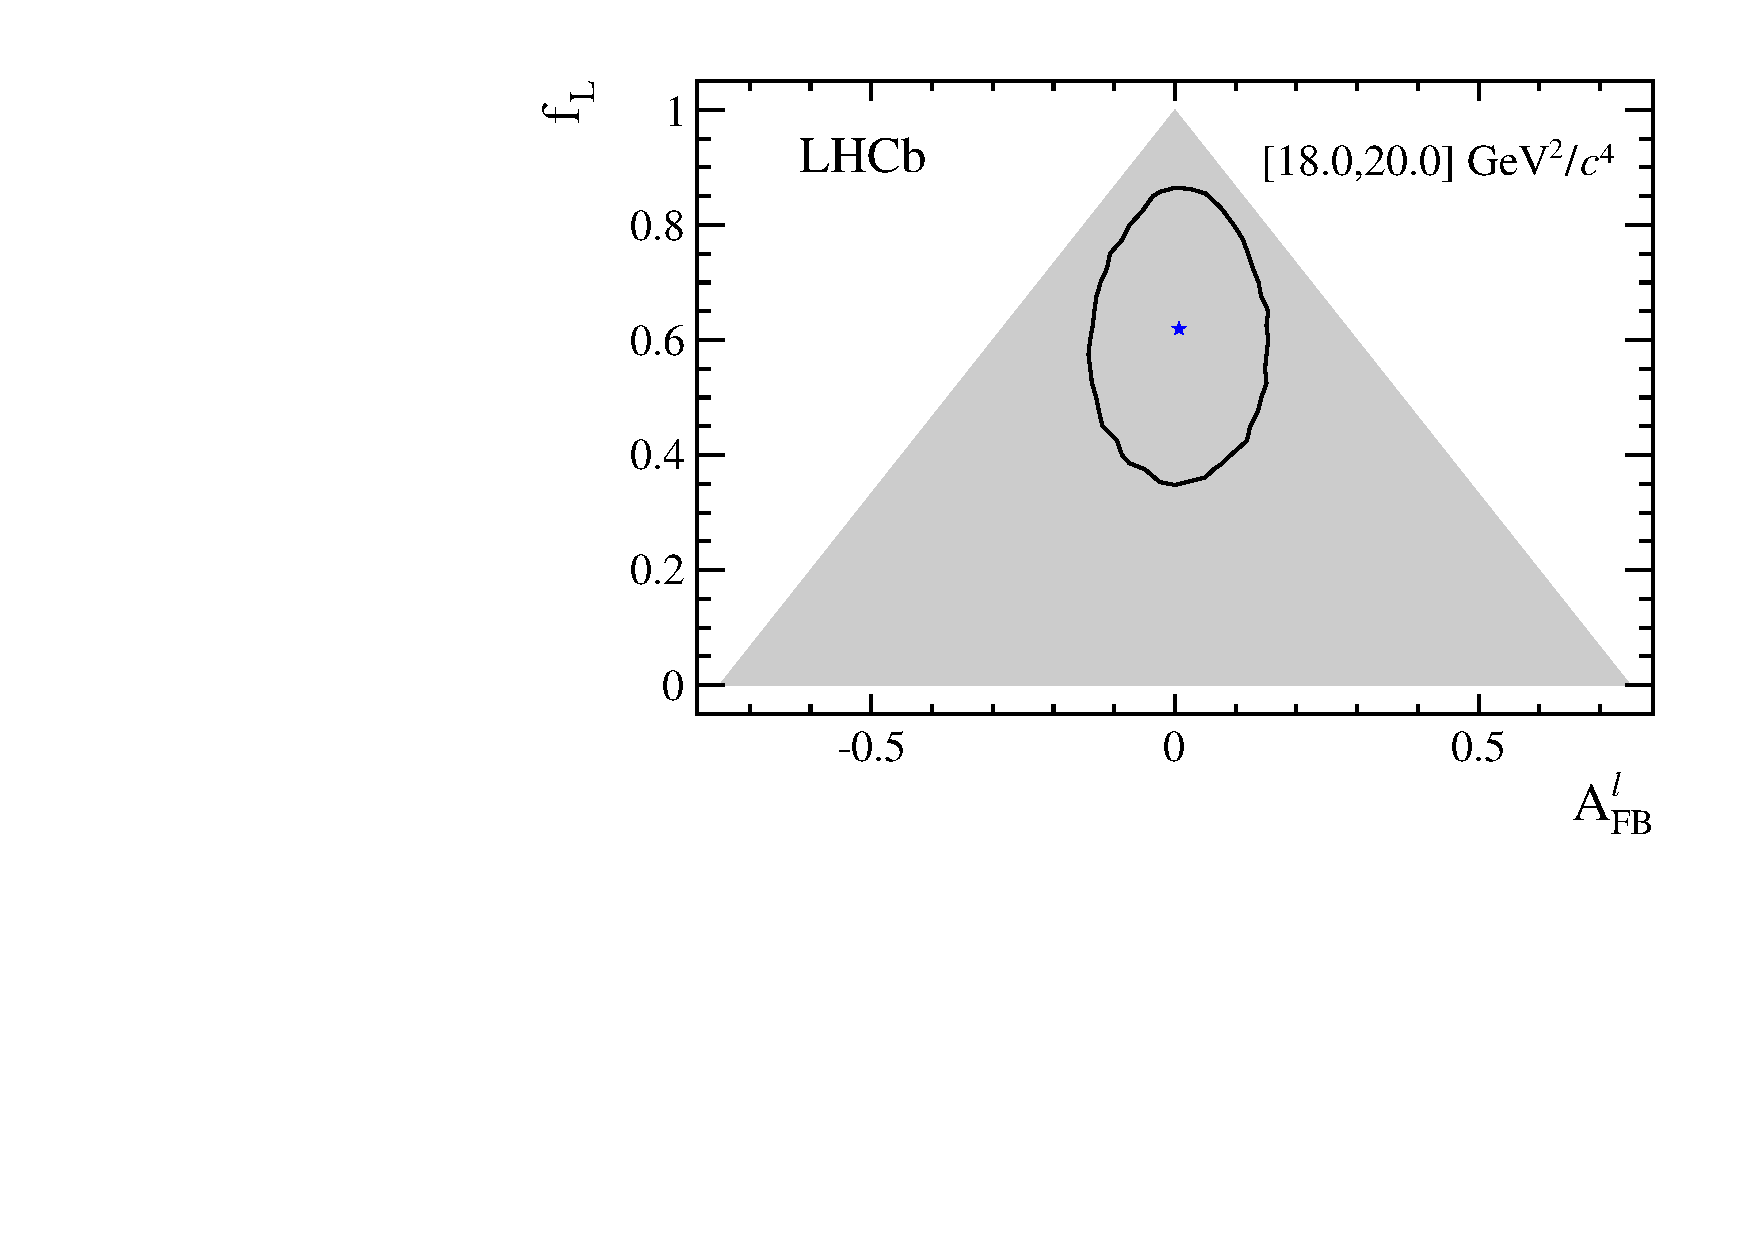
\includegraphics[width=0.49\textwidth]{figure10e.pdf}
\caption{Two-dimensional 68\,\% CL regions (black) as a
  function of $A_{\rm FB}^\ell$ and $f_{\rm L}$.  The shaded areas
  represent the regions in which the PDF is positive over the complete $\cos
  \theta_{\ell}$ range. The best fit points are indicated by the (blue) stars. }
\label{fig:contours}
\end{figure}

The two-dimensional 68\,\% CL regions for the observables 
$A_{\rm FB}^\ell$ and $f_{\rm L}$ are given in Fig~\ref{fig:contours},
for each \qsq interval in which signal is observed.
